\documentclass[a4paper,twocolumn]{article}

\usepackage[english]{babel}
\usepackage[utf8]{inputenc}
\usepackage{graphicx}
\usepackage{fullpage}

\usepackage{titlesec}

\titleformat*{\section}{\large\bfseries}
\titleformat*{\subsection}{\normalsize\bfseries}


\title{Distilling the Knowledge in a Neural Network $-$ summary}
\author{Matěj Nikl}

\begin{document}
\maketitle
A process called \textit{distillation} is a kind of learning that can be used to transfer a knowledge from a cumbersome model (or an ensemble of models) to a smaller/single model, which is more suitable for deployment, while preserving the knowledge and thus preserving the performance.

To do so, the standard back-propagation algorithm (with a different objective function) is used.

\section{Softmax with temperature}
Neural networks typically produce class probabilities by using a \textit{softmax} output layer that converts the logit, $z_i$, computed for each class into a probability, $q_i$, by comparing $z_i$ with the other logits
\[
    q_i = \frac{e^{z_i/T}}{\sum_j e^{z_j/T}}
\]
where a temperature $T$ is normally set to 1. Using a higher value for $T$ produces a softer probability distibution over classes.

\section{Distillation}

A side-effect of learning is that a trained model assigns probabilities to all of the incorrect answers and even when these probabilities are very small, some of the are much larger than others $-$ the relative probabilities of incorrect answers tell us a lot about how the model tends to generalize. An image of a car, for example, may only have a very small chance of being mistaken for a truck, but that mistake is still much more probable than mistaking it for an apple.

By using all the class probabilities produced by a cumbersome model as \textit{soft targets} for a small model, the knowledge can be transferred. For this transfer stage, the same training set or even a different \textit{transfer} set can be used. For an ensemble of models, an arithmetic or geometric mean of their individual predictive distributions as the soft targets can be used. Moreover, when the soft targets have high entropy, they provide much more information per training case than hard targets and much less variance in the gradient between training cases, so the small model can often be trained on much less data and using a much higher learning rate.


\paragraph{The gradient to match the soft target}
Each case in the trasfer set contributes a cross-entropy gradient, $dC/dz_i$, with respect to each logit, $z_i$ of the distilled model. If the cumbersome model has logits $v_i$ which produce soft target probabilities $p_i$ and the transfer training is done at a temperature of $T$, this gradient is given by:
\[
    \frac{\partial C}{\partial z_i} = \frac{1}{T}(q_i - p_i) = \frac{1}{T}\left( \frac{e^{z_i/T}}{\sum_j e^{z_j/T}} - \frac{e^{v_i/T}}{\sum_j e^{v_j/T}} \right)
\]
If the temperature is high compared with the magnitude of the logits, we can approximate ($e^x \approx 1+x$ for small $x$):
\[
    \frac{\partial C}{\partial z_i} \approx \frac{1}{T}\left( \frac{1 + z_i/T}{N + \sum_j z_j/T} - \frac{1 + v_i/T}{N + \sum_j v_j/T} \right)
\]
If we now assume that the logits have been zero-meaned separately for each transfer case so that $\sum_j z_j = \sum_j v_j = 0$, we can further simplify to:
\[
    \frac{\partial C}{\partial z_i} \approx \frac{1}{NT^2} (z_i - v_i)
\]

% It is done by:
% \begin{enumerate}
%     \item having a model (or an ensemble of models) to transfer the knowledge from
%     \item
% \end{enumerate}



% \begin{figure}[!h]
%     % \centering
%     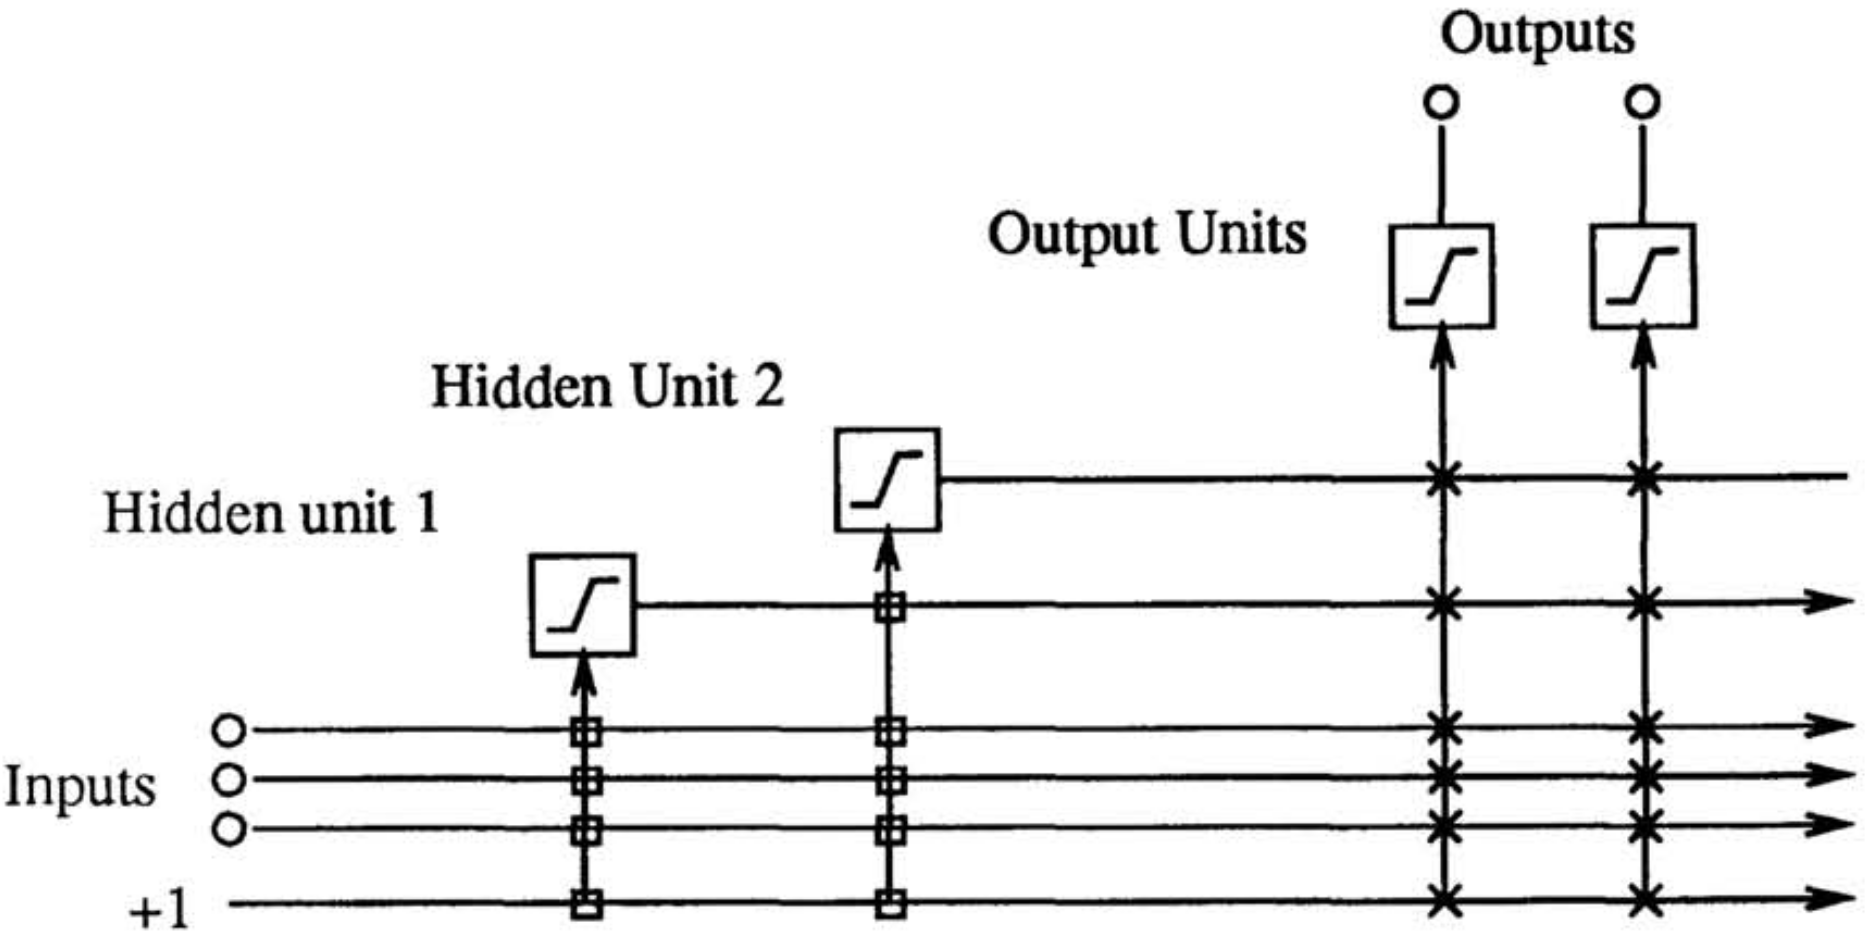
\includegraphics[width=0.475\textwidth]{cascade.png}
%     \caption{The CCA after two hidden units have been added. The vertical lines sum all incoming activations. Boxed connections are frozen, X connections are trained repeatedly.}
% \end{figure}

% \section{Principles of modularization}
% \section{Principles of growing}
% The only sense of modularization in the CCA can be seen in viewing individual hidden units as modules, since they are being added throughout the learning process. However, the network as a whole is not modular in the full sense. Hidden units cannot be detached from a network and reattached to a different one. A hidden unit can only be used in conjunction with the hidden units it has been trained with and nowhere else.
\end{document}
